\documentclass{article}

% Language setting
% Replace `english' with e.g. `spanish' to change the document language
\usepackage[english]{babel}

% Set page size and margins
% Replace `letterpaper' with `a4paper' for UK/EU standard size
\usepackage[letterpaper,top=2cm,bottom=2cm,left=3cm,right=3cm,marginparwidth=1.75cm]{geometry}

% Useful packages
\usepackage{amsmath}
\usepackage{graphicx}
\usepackage[colorlinks=true, allcolors=blue]{hyperref}

\title{Project 611 Report -- Prediction on EPL Games and Some Interesting Facts about EPL}
\author{Meisheng Xiao 730423061}

\begin{document}
\date{}
\maketitle


\section{Introduction}
This project utilizes data from the English Premier League (EPL) spanning the seasons from 2009 to 2022. The EPL is one of the most competitive soccer leagues on Earth and the most lucrative soccer league in the world. Beginning in 2009, the EPL entered a new era, often referred to as the “golden era” by fans, characterized by significant investments from wealthy investors. During this period, 39 teams have competed in the EPL. Among these, six teams, known as the “Big 6” due to their outstanding performance, are Arsenal, Chelsea, Liverpool, Manchester City, Manchester United, and Tottenham Hotspur.
The aim of this project is to create models to predict game outcomes and potentially leverage these predictions for betting. However, due to the constraints of the final week, I have only developed one multinomial logistic regression model for prediction and have not created a linear optimizer for the betting aspect. Additionally, this project includes interesting data visualizations and interpretations.
Dataset: Original dataset is downloaded from \href{https://www.kaggle.com/datasets/saife245/english-premier-league}{there}. The original data contain 20 years of EPL(English Premier League) results data. Basically, the data contains each game’s result statistics of 20 years. I take data started from 09-10 season as they started to have a bet ratio from gambling company. After some data cleaning(Code please see “source\_data/data\_cleaning.R"), I create a more compact dataset which includes many variables I think is relevant with the result of a game (detailed description is source\_data/data\_description.txt).

\section{Home Team Performance and Home Stadium Effects}

\begin{figure}[h!]
\centering
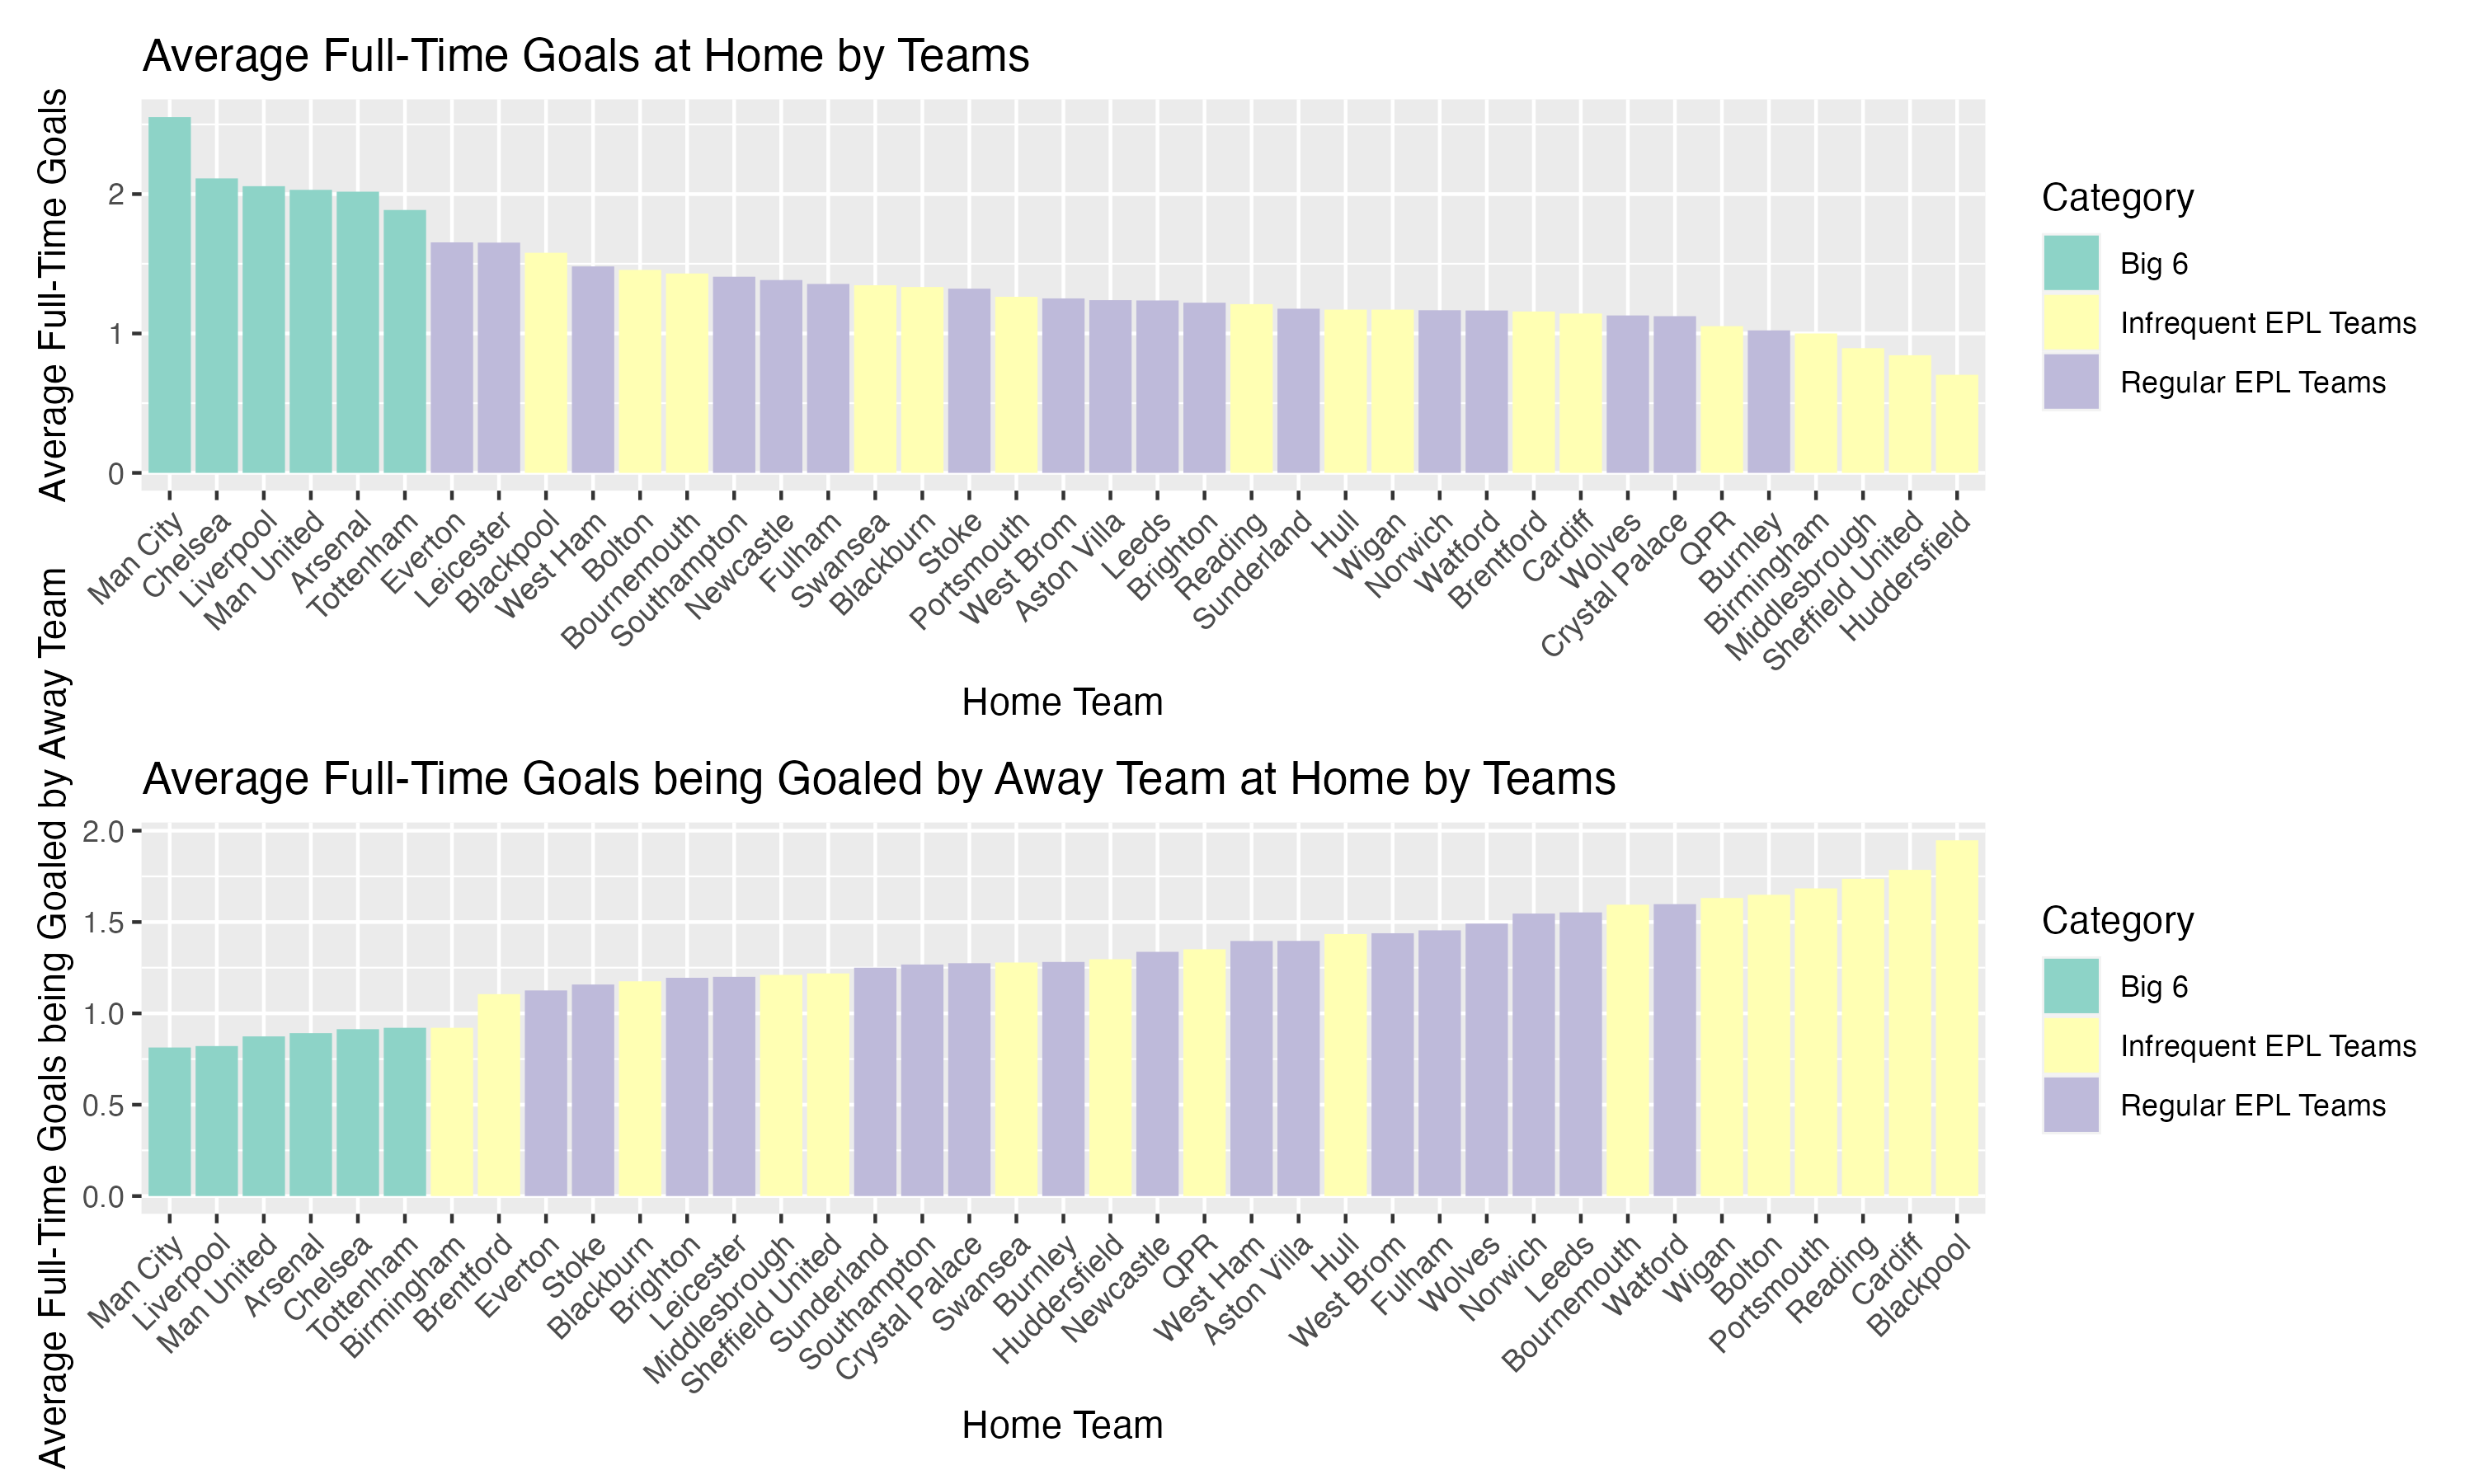
\includegraphics[width=\textwidth]{HomeTeam_performance.png}
\caption{\label{fig:htp}Home Team Performance}
\end{figure}

Figure \ref{fig:htp} displays two bar plots. The top plot shows the average number of full-time goals scored by teams in their home games, while the bottom plot shows the average number of full-time goals scored against them in their home games.

In soccer, home stadiums can significantly impact a team's performance, often influenced by local fan culture. These plots represent the performance of home teams in their respective stadiums. The data indicates that Manchester City has the most formidable home stadium atmosphere, with an average of 2.5 goals scored in home games and the lowest likelihood of conceding goals. Among the Big 6, Tottenham has the weakest home advantage, aligning with their perception as the least dominant team in the Big 6.

Teams outside the Big 6 typically have lower average goals and a higher likelihood of being scored, reflecting a realistic trend. The Big 6, however, exhibit the most successful home atmosphere.

\section{Who is the Real Boss between Big 6}

\begin{figure}[h!]
\centering
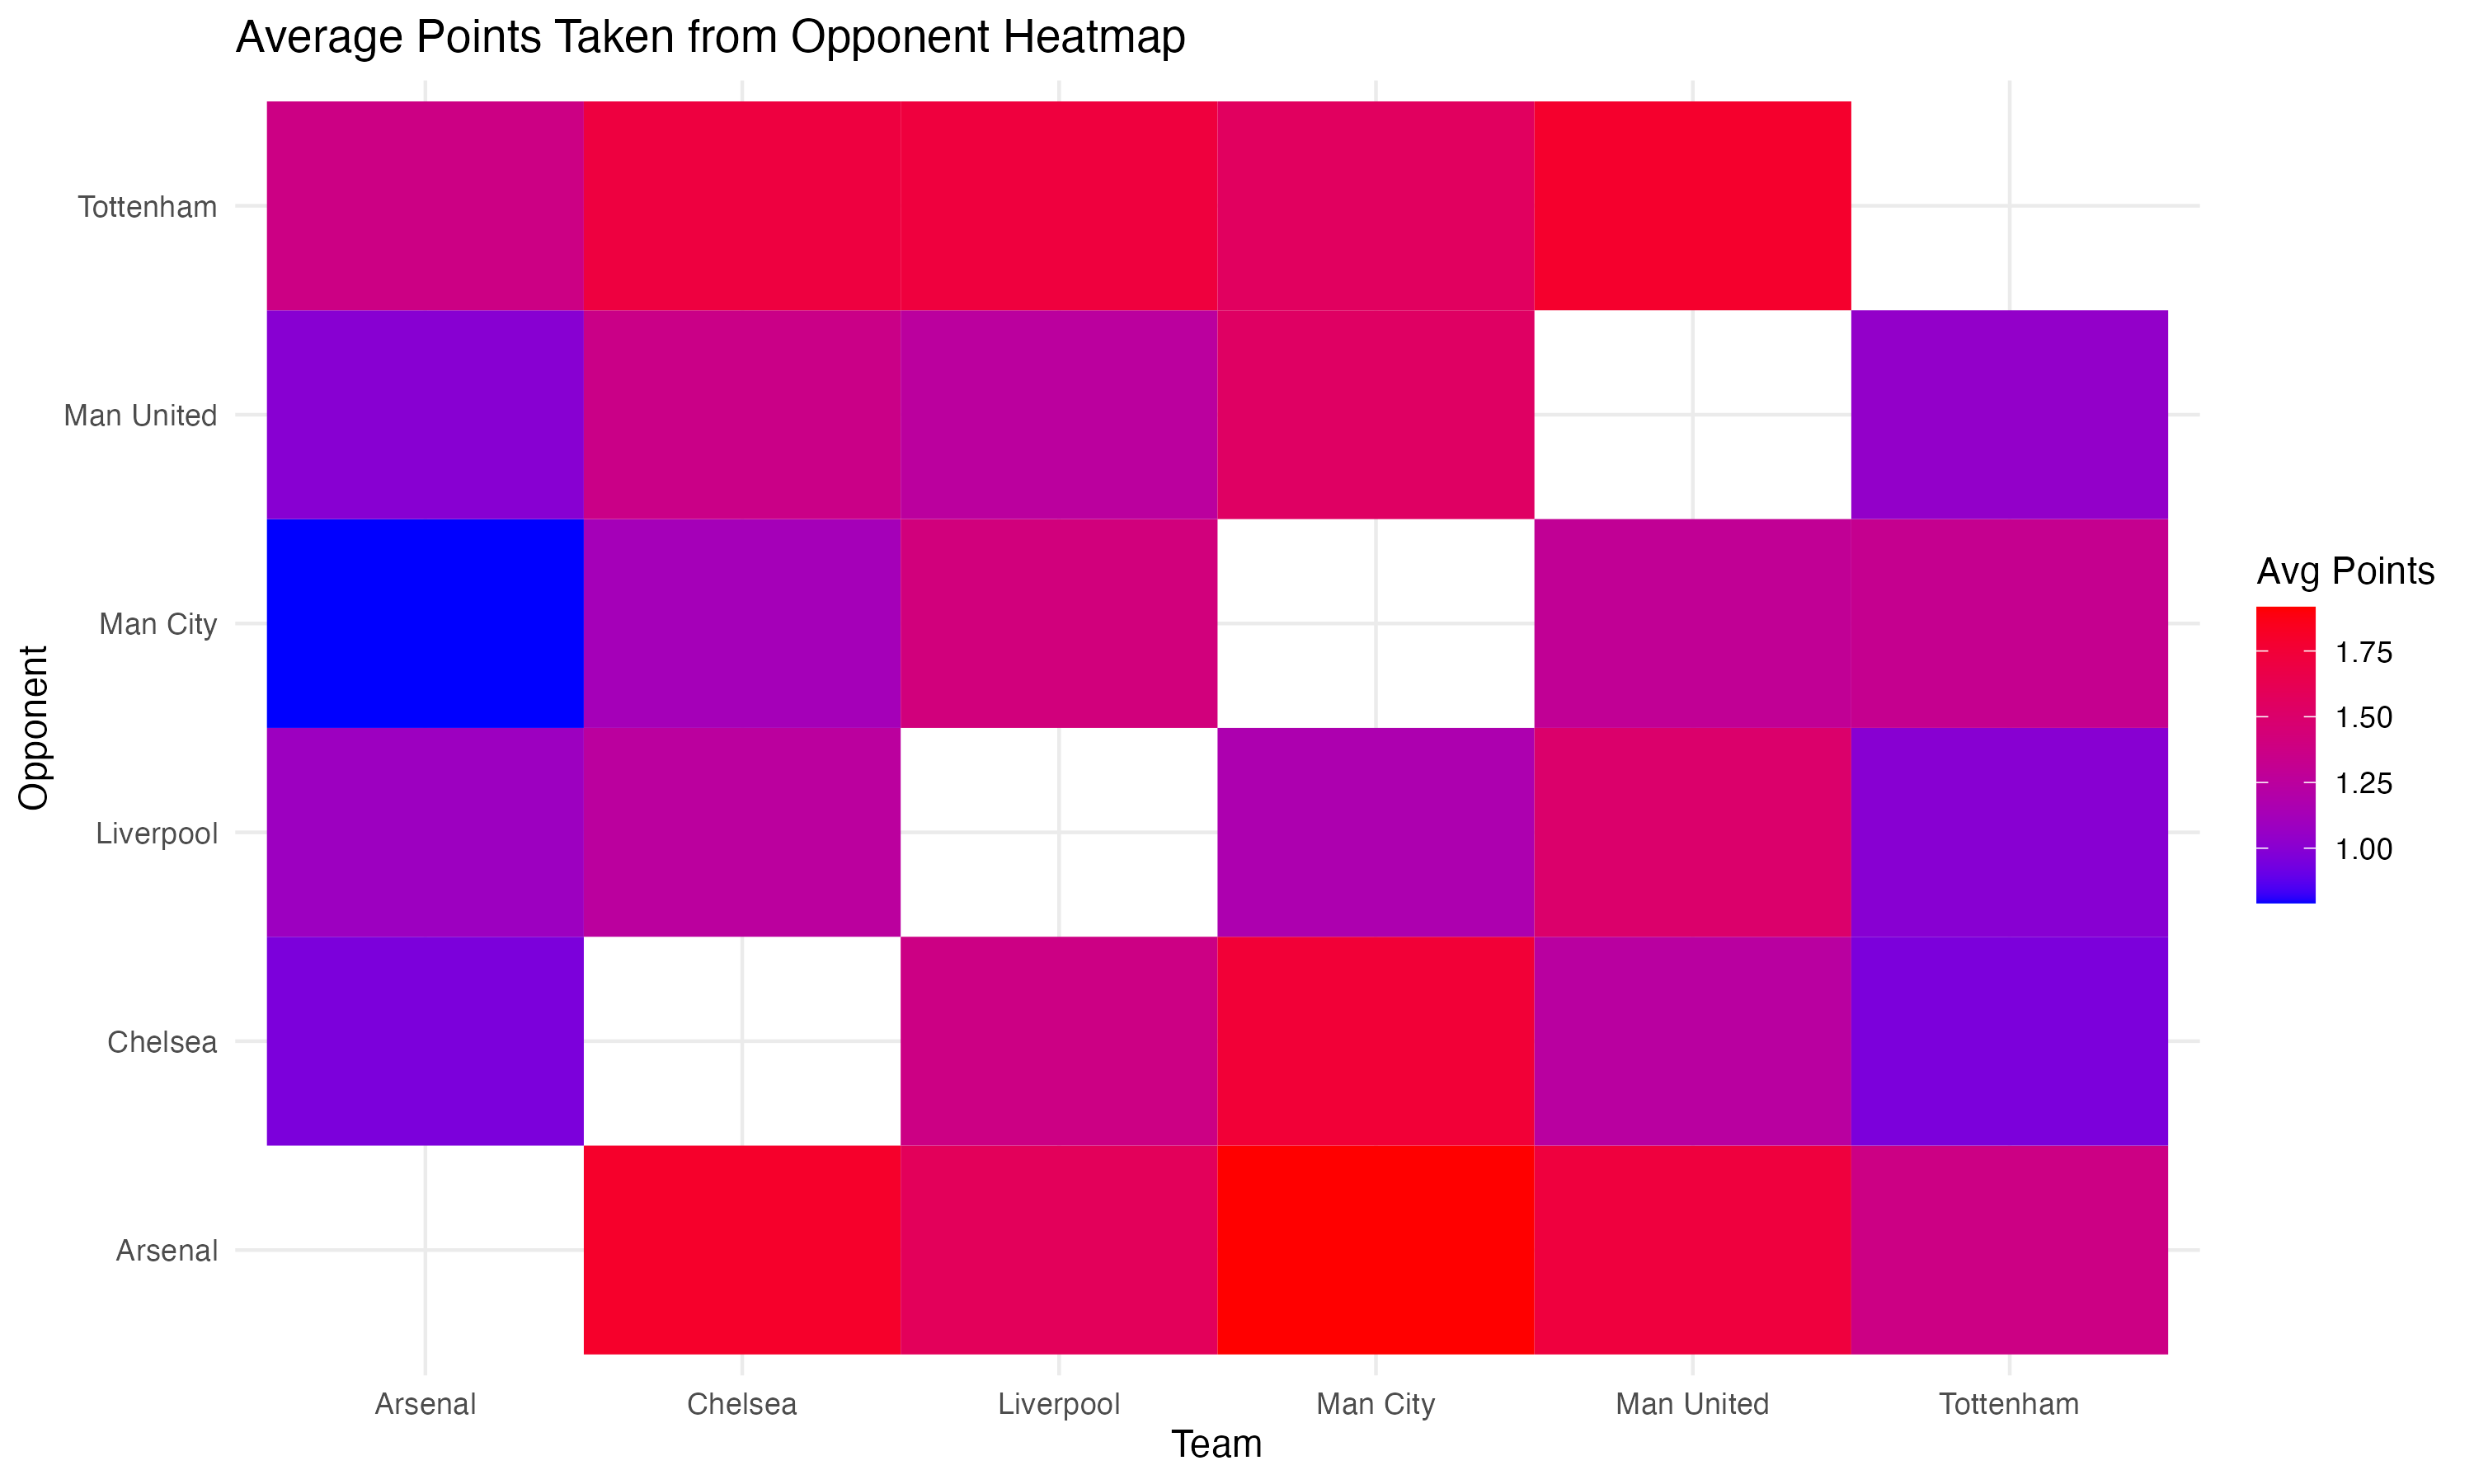
\includegraphics[width=\textwidth]{avg_points_heatmap_big6.png}
\caption{\label{fig:heatmap}Performance between Big 6}
\end{figure}

Matches between the Big 6 teams always captivate soccer fans, representing high-end competition. This heatmap \ref{fig:heatmap} provides information on the average points that a Big 6 team can secure from matches against other Big 6 teams, revealing the dominant force within this elite group. The EPL point system awards 3 points for a win, 1 point for a draw, and 0 points for a loss. Consequently, the average points taken from these encounters randomly is 1.333 points per team.

The heatmap \ref{fig:heatmap} reveals that Arsenal is the weakest in competitions among Big 6, with dominance exerted over them by all except Tottenham. This might be attributed to the Arsenal-Tottenham rivalry, known as the London Derby, where Arsenal historically elevates its performance.
Manchester City emerges as the big boss among the Big 6, dominating all but Liverpool. Liverpool's resilience is world-known, attributed to their renowned spirit and stamina.

\section{Public Opinions via Bet Ratio}

\begin{figure}[h!]
\centering
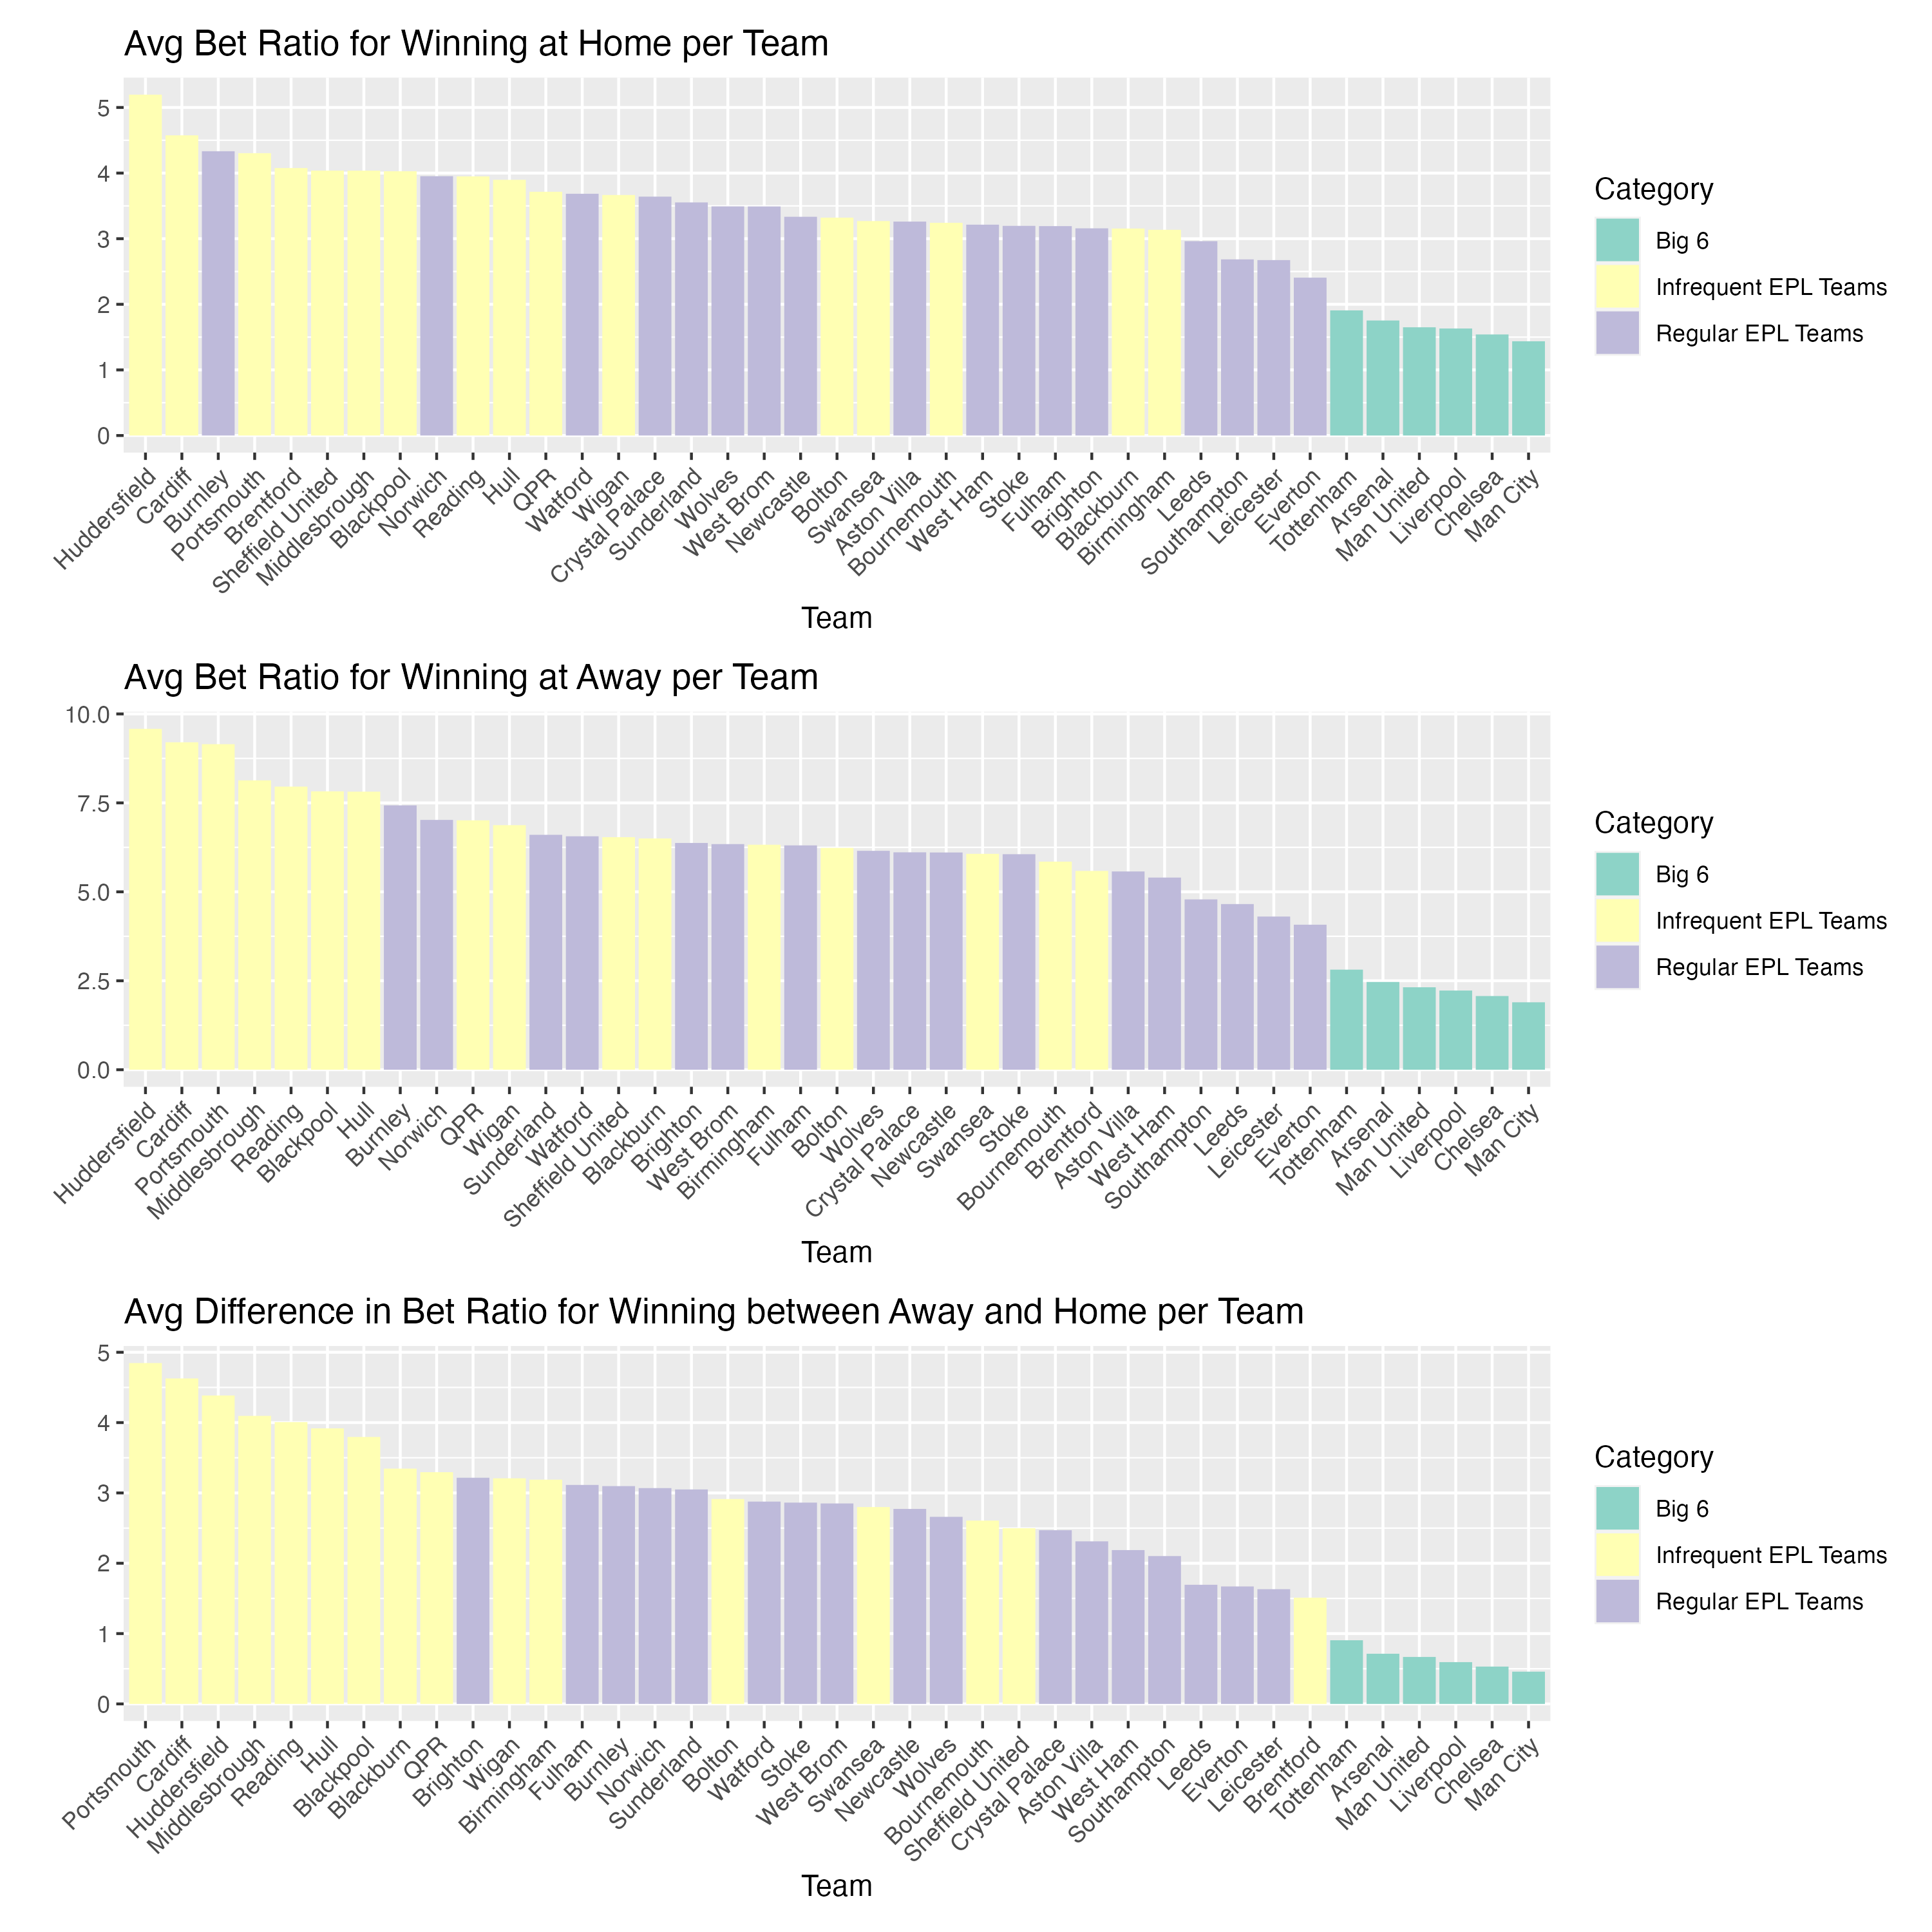
\includegraphics[width=\textwidth]{BetRatio.png}
\caption{\label{fig:betratio}Bet Ratio for 39 Teams}
\end{figure}

This figure \ref{fig:betratio} comprises three bar plots. The top plot shows the average betting ratio for home wins for each team, the middle plot for away wins, and the bottom plot depicts the difference in average betting ratios between home and away wins. As betting companies aim to maximize profits, these ratios offer insight into public perceptions of each team. Hence, the bet ratios somewhat reflect public opinion.

Manchester City, Chelsea, Liverpool, and Manchester United are perceived as the most successful teams, which aligns with their track records. Domestically, these teams have collectively won 12 championships in the past 13 seasons. Internationally, they have frequently reached the UEFA Champions League finals, with Manchester City, Chelsea, and Liverpool winning the title in the last 13 years, signifying their status as world-class teams.
Brentford, interestingly, is perceived as having a relatively stronger away performance and weaker home performance. Without extensive knowledge of Brentford's history, the reason for this perception remains intriguing but unclear.

\section{Fouls, Yellow and Red Cards}
In soccer, fouls represent illegal moves that offer unfair advantages or exhibit unsportsmanlike behavior. Severe fouls can result in yellow or red cards from the referee, serving as warnings or penalties. Accumulating two yellow cards or receiving a red card results in a player's immediate expulsion from the game. Therefore, the average number of fouls, yellow cards, and red cards per game for each team is of interest to determine if certain teams exhibit more physical or violent play styles than others over the selected 13 seasons.

\begin{figure}[h!]
\centering
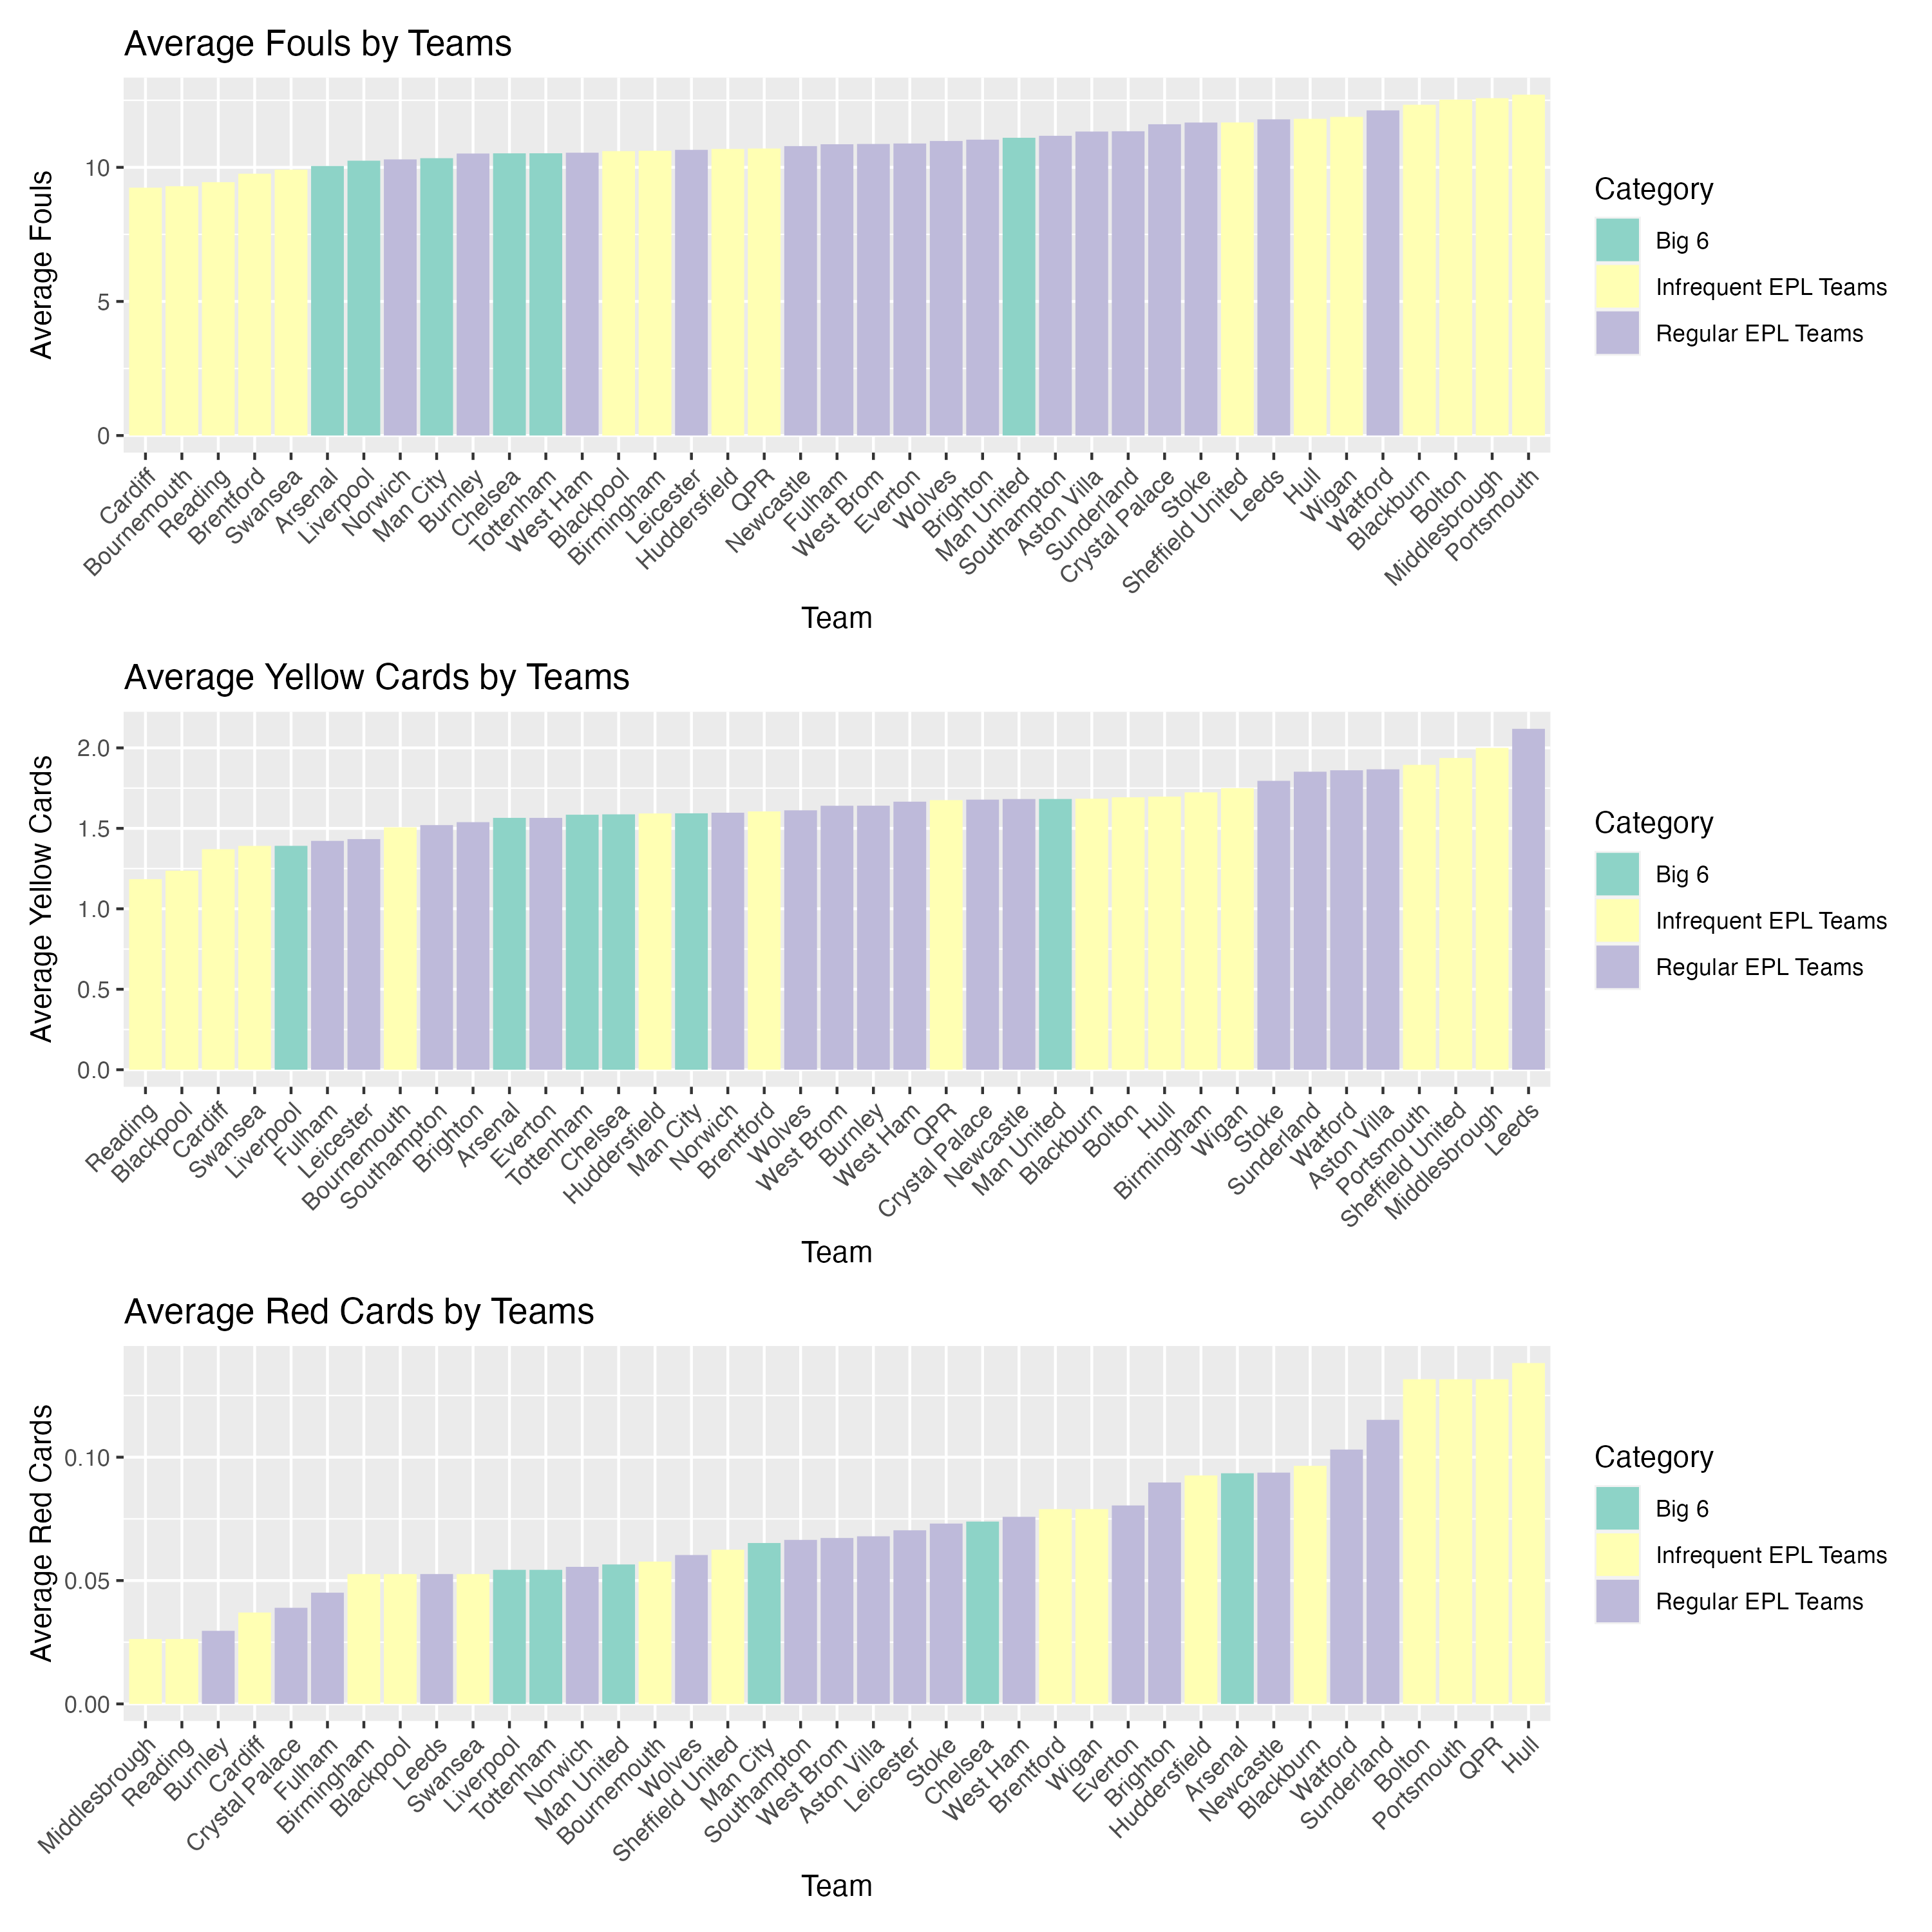
\includegraphics[width=\textwidth]{Team_Fouls.png}
\caption{\label{fig:fouls}Fouls, Yellow and Red Cards}
\end{figure}

The figure \ref{fig:fouls} includes three bar plots: the average number of fouls, yellow cards, and red cards per team. Arsenal, within the Big 6, interestingly records the lowest number of fouls and the second-lowest number of yellow cards, but a significantly higher number of red cards. This could suggest that Arsenal players tend to receive red cards early in games, reducing their overall foul and yellow card averages as the team will continue playing with one player less. In contrast, Leeds United appears to play physically but strategically, evidenced by a relatively high rate of fouls and yellow cards but a low rate of red cards.

\section{Multinomial Logistic Regression Part}
Data from 11 seasons (2009 to 2020) were used as training data, with data from the following two seasons (2020 to 2022) serving as the test set. Various data cleaning steps were implemented (see data\_cleaning.R for details). The model use covariates representing each team's performance in their last three games.

A multinomial logistic regression model predicts game outcomes (home win, away win, or draw). The model's accuracy in the test set is 0.4859, a significant improvement over random guessing, which has an accuracy of 0.3333.

\section{Future Questions \& Analysis}
The plan was to create a gambling model. The expectation of mine is to create a two-part hierarchical model. I have finished the first-part model, a classifier that can predict a game’s result. I actually tried three classifiers, which are multinomial logistic regression, random forest, and neural networks. Among these three models, multinomial logistic regression won, with an accuracy of 0.486 on the test set, while the other two models give accuracies below 0.48 on the test set. Further refinement on the multinomial logistic regression can be made on feature selection to make predictions easier.

The second-part model would be a linear optimizer that can give an optimal betting strategy that has the best expectation of profit from betting the results of games per round. There are no technical problems with the linear optimizer as it is easy and quick to solve and valid in theory. However, how to set a reasonable gambling strategy to create the objective function (loss function) and constraints for the linear optimizer needs some considerations. Now I have one idea about the strategy. Using the product of predicted probability and bet ratio as my decision criteria, which will show the expected gaining ratio. When the expected gaining ratio is bigger than 1, it means I can earn money from the game on average. The decision for this strategy will be to bet money in the predicted probability ratio into each result if the expected gaining ratio is bigger than 1.5.


\end{document}